\section{Review of TDL extrapolations}
\begin{frame}
    \frametitle{LDA+GW}
    \begin{figure}
        \centering
        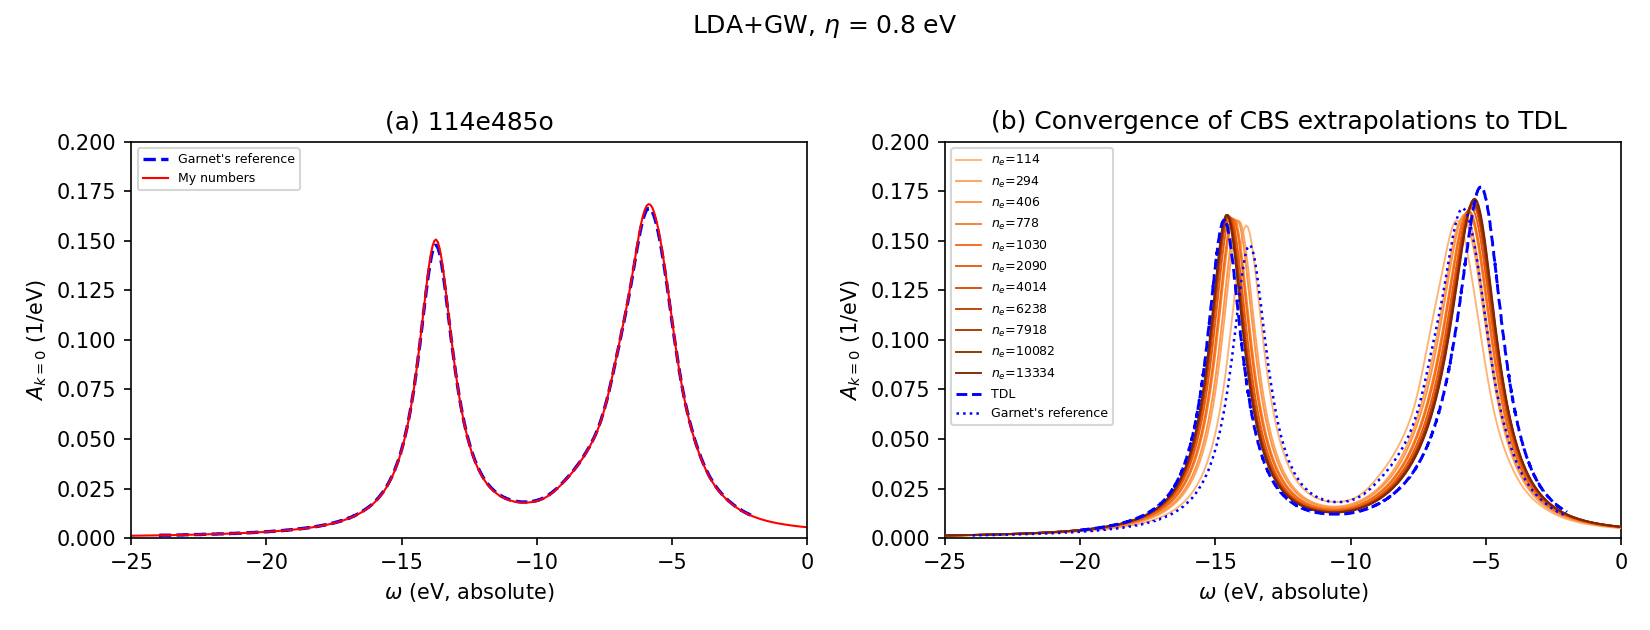
\includegraphics[width=\textwidth]{26/8/8-07/mcclain_compare.png}
        % \caption{LDA+GW}
    \end{figure}
\end{frame}
\begin{frame}
    \frametitle{LDA+GW+C Garnet's convention}
We are using 
\begin{equation}
    C_k^R(t) = \frac{1}{\pi}\int d\omega \frac{|\operatorname{Im} \Sigma^R_k(\omega+{E^{GW}_k})|}{\omega^2} \left( e^{-i\omega t} + i\omega t - 1 \right).
\end{equation}
\pause
    \begin{figure}
        \centering
        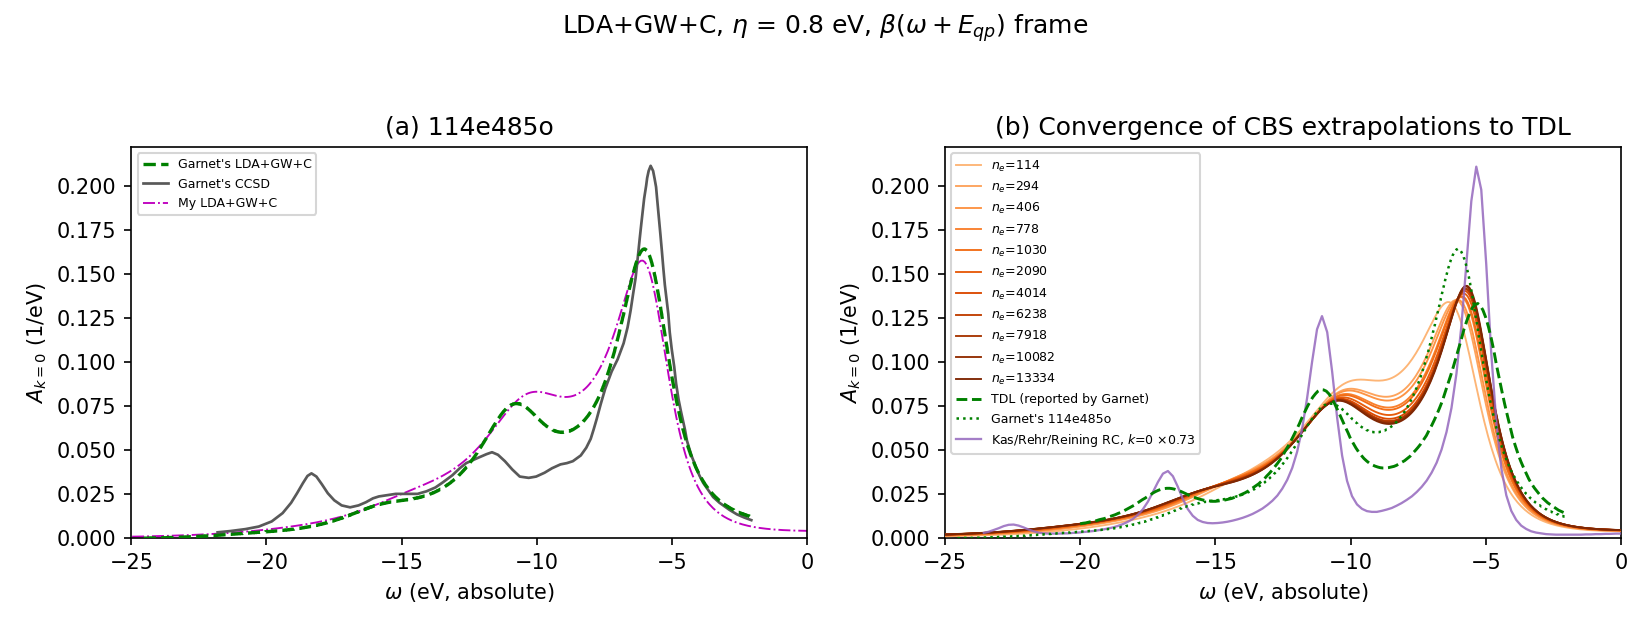
\includegraphics[width=\textwidth]{26/8/8-07/mcclain_gwc_compare_eqp.png}
        % \caption{LDA+GW}
    \end{figure}
% In the $\beta(\omega+E_{QP})$ and $\beta(\omega+\epsilon_{\mathrm{LDA}})$ frames, we are using $\epsilon_k \equiv E_k^{GW} $ and $\epsilon_k \equiv \epsilon_k^{\mathrm{LDA}}$, respectively.

\end{frame}
\begin{frame}
    \frametitle{LDA+GW+C Garnet's convention continued}
    \begin{figure}
        \centering
        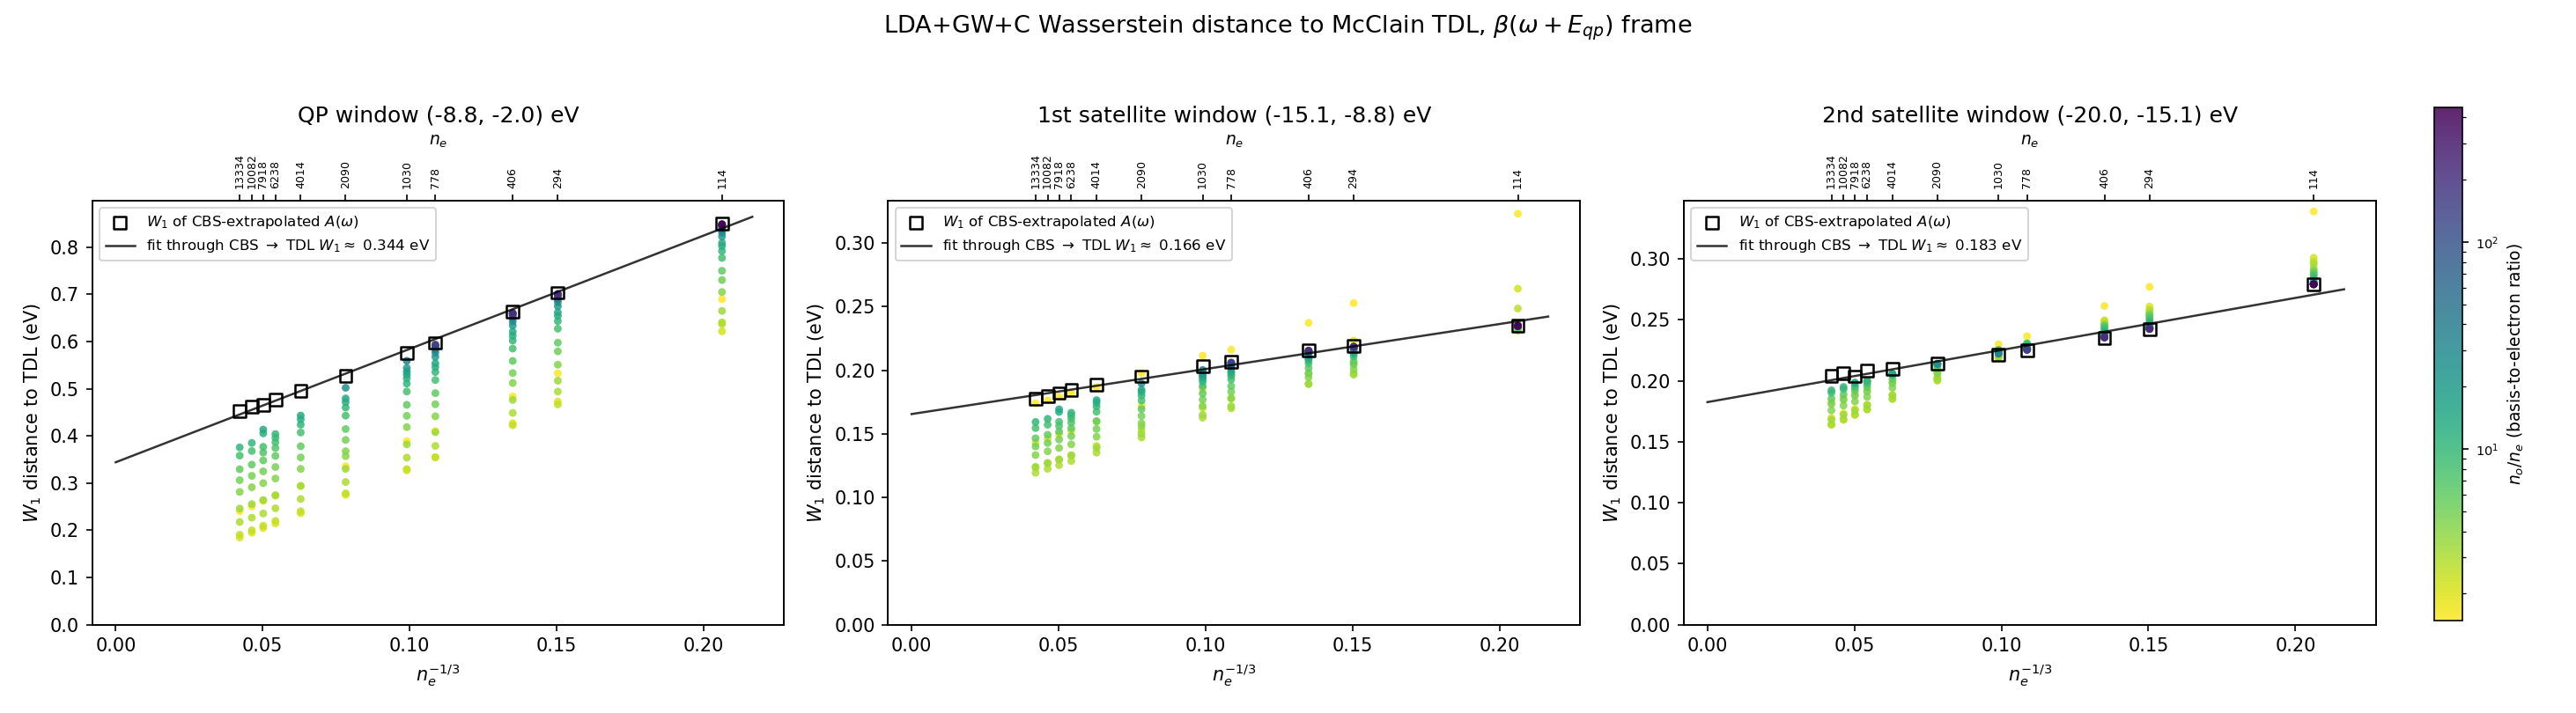
\includegraphics[width=\textwidth]{26/8/8-07/mcclain_gwc_wasserstein_eqp.png}
        % \caption{LDA+GW}
    \end{figure}
\end{frame}
\begin{frame}
    \frametitle{LDA+GW+C Loos' convention}
We are using 
\begin{equation}
    C_k^R(t) = \frac{1}{\pi}\int d\omega \frac{|\operatorname{Im} \Sigma^R_k(\omega+{\epsilon^{LDA}_k})|}{\omega^2} \left( e^{-i\omega t} + i\omega t - 1 \right).
\end{equation}
\pause
    \begin{figure}
        \centering
        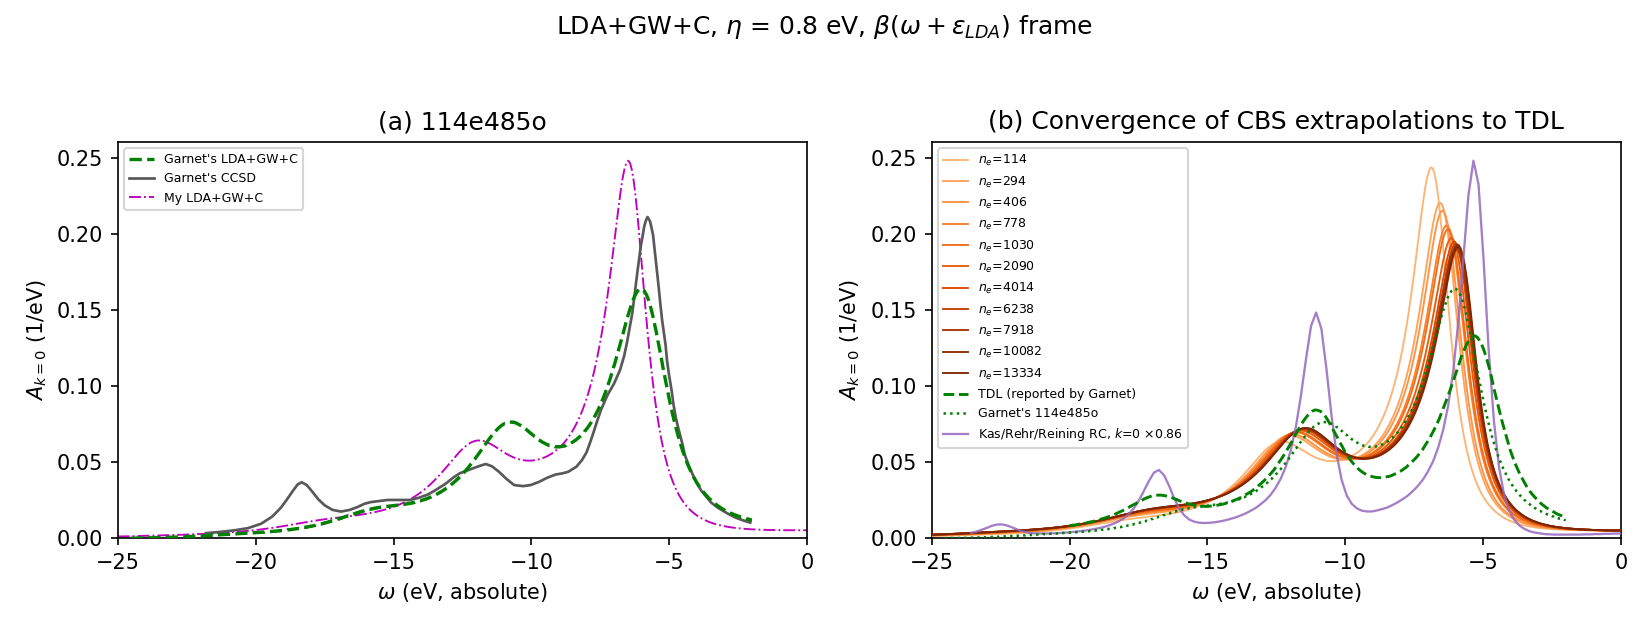
\includegraphics[width=\textwidth]{26/8/8-07/mcclain_gwc_compare.png}
        % \caption{LDA+GW}
    \end{figure}
\end{frame}
\begin{frame}
    \frametitle{LDA+GW+C Loos' convention continued}
    \begin{figure}
        \centering
        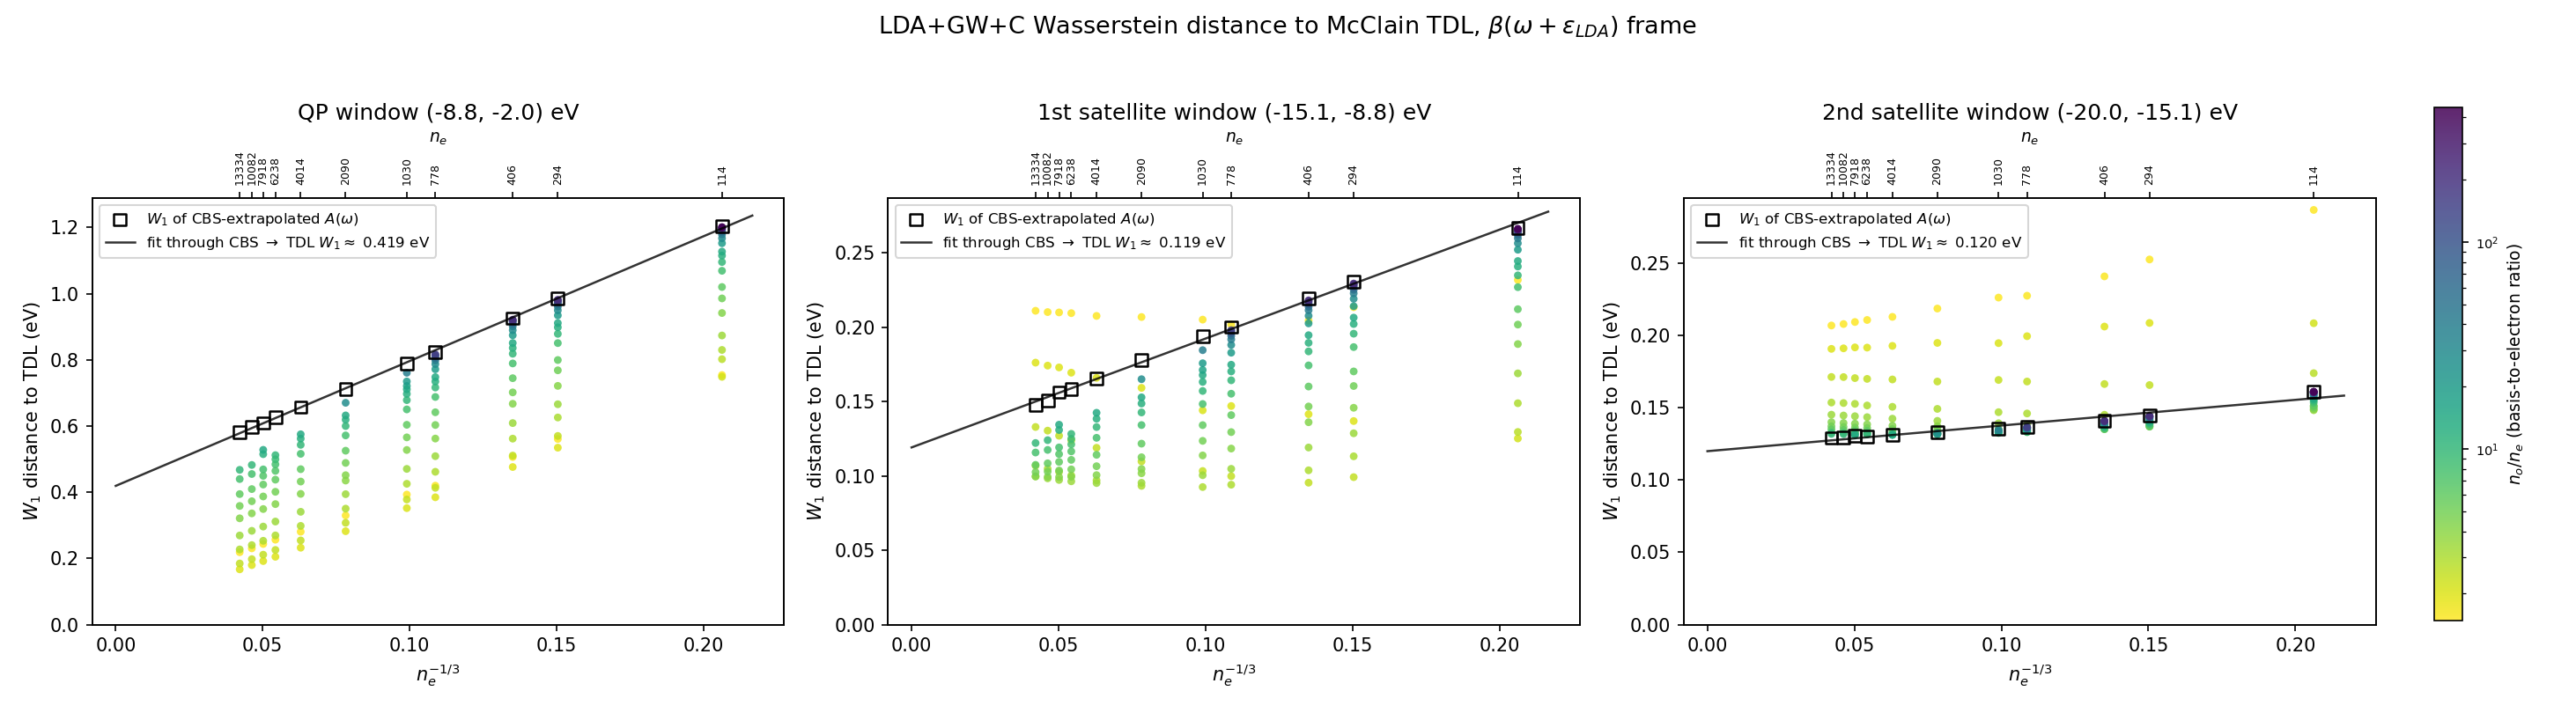
\includegraphics[width=\textwidth]{26/8/8-07/mcclain_gwc_wasserstein.png}
        % \caption{LDA+GW}
    \end{figure}
\end{frame}
\section{What to do next}
\begin{frame}
    \frametitle{What I have done so far}
\begin{enumerate}
\item Reproduced Garnet's LDA+GW curve for 14e19o and 114e485o \pause
    \begin{itemize}
        \item Wrote an LDA code for the UEG that we verified against PySCF \pause
        \item Wrote a GW code for the UEG that we verified against PySCF \pause
    \end{itemize}
\item Reproduced Loos' finite basis HF+GW+C curves for molecules \pause
    \begin{itemize}
        \item This was only for valence states and not using LDA reference \pause
    \end{itemize}
\item Told Claude Code about all the above and asked it to reproduce Garnet's finite basis LDA+GW+C, but nothing came close \pause   
\end{enumerate}
What should we do next?
\end{frame}

\section{Applying dCC to the UEG spectral function}
\begin{frame}
    \frametitle{How I think we could apply dCC ideas to the UEG spectral function}
Consider
\begin{equation}
H_p^{\rm eff}
=
\epsilon_p^{\rm MF} a_p^{\dagger} a_p
+
\sum_{m\nu}
\Delta_{pm\nu}
B_{pm\nu}^{\dagger}
B_{pm\nu}
+ a_p^{\dagger} a_p
\sum_{m\nu}
\left(
\mathcal{M}_{pm\nu}
B_{pm\nu}^{\dagger}
+
\mathcal{M}_{pm\nu}^{*}
B_{pm\nu}
\right),
\end{equation}
with QB operators $B_{pm\nu}^{\dagger}$. \pause
$\Delta_{pm\nu} = \epsilon_p^{\rm MF} - \epsilon_m^{\rm MF} + \operatorname{sgn}(\epsilon_m^{\rm MF} - \epsilon^{\rm MF}_{k_F})\Omega_\nu$ and $\mathcal{M}_{pm\nu}$ are QB excitation energies and couplings, respectively. \pause
This is used to obtain Green's functions for GW+C and PT2+C. \pause It seems to me that in order to get Hamlin's dCC, instead of getting bosonic quantites from the QBA, one gets them with DFPT.
\end{frame}
